% *{{ All Setup
% *{{ preamble
\documentclass[12pt, pdf, hyperref={draft}, usenames, dvipsnames,
aspectratio=169]{beamer}
\usepackage{libertine, textcomp, amssymb, wasysym, color, ulem, verbatim}
\usepackage{floatrow, subcaption}
% hide controls
\usenavigationsymbolstemplate{}
\usepackage[T1]{fontenc}
\synctex=1
\setbeamertemplate{caption}[numbered]

% can use later to change the margin size, if want.
% \setbeamersize{text margin left=10pt,text margin right=10pt}

% }}*

% *{{ item colouring and themes
\usecolortheme{beaver}
\setbeamertemplate{footline}[frame number]
\definecolor{LancsRed}{HTML}{B5121B}
\setbeamercolor{item}{fg=LancsRed}
\setbeamercolor{title}{fg=LancsRed}
\setbeamercolor{structure}{fg=LancsRed}
\setbeamercolor{frametitle}{fg=LancsRed}
\setbeamercolor{footnote mark}{fg=LancsRed}
\setbeamercolor{footnote}{fg=LancsRed}
\setbeamercolor{bibliography entry author}{fg=LancsRed}
\setbeamercolor{bibliography entry title}{fg=black}
\setbeamercolor{bibliography entry note}{fg=black}
\setbeamercolor{section in toc}{fg=LancsRed}
%\setbeamercolor{subsection in toc}{fg=gray}
\newcommand{\gitem}[1]{\setbeamercolor{item}{fg=ForestGreen}\item[$\checkmark$] #1}
\newcommand{\bitem}[1]{\setbeamercolor{item}{fg=LancsRed}\item[$\times$] #1}
\newcommand{\nitem}[1]{\setbeamercolor{item}{fg=NavyBlue}\item[$-$] #1}
% }}*

% *{{ niceties
\newcommand{\dd}{\mathrm{d}}
\newcommand{\e}{\mathrm{e}}
\newcommand{\ket}[1]{\lvert{#1}\rangle}
\newcommand{\bra}[1]{\langle{#1}\rvert}
\newcommand{\expt}[1]{\langle{#1}\rangle}
\newcommand{\red}[1]{{\bf\color{LancsRed}{#1}}}
\newcommand{\blue}[1]{{\bf\color{NavyBlue}{#1}}}
\newcommand{\green}[1]{{\bf\color{ForestGreen}{#1}}}
\newcommand{\pt}{\Psi_{\text{T}}}
\newcommand{\tpt}{{\tilde\Psi}_{\text{T}}}

% }}*

% *{{ title, subtitle, inst., date
\title{Excited States by Quantum Monte Carlo}
\subtitle{QMC in the Apuan Alps 2017}

% authors and institutions
%\author{\emph{Ryan J. Hunt}\inst{1},
%        Neil D. Drummond\inst{1} \\
%        and Vladimir I. Fal'ko\inst{2}}

\author{Ryan J. Hunt\\
        Lancaster University}

%\institute[]{
%
%  \inst{1}
%  Department of Physics,\\
%  Lancaster University
%  \and
%
%  \inst{2}
%  National Graphene Institute,\\
%  University of Manchester}
%
% date
\date{4$^{\text{th}}$ August 2017}

% }}*

% *{{ bibliography setup
\usepackage[backend=bibtex, style=phys]{biblatex}
\bibliography{exc_refs}
\renewcommand{\footnotesize}{\scriptsize}
\AtEveryCitekey{\clearfield{title}
                \clearfield{pagetotal}
                \clearfield{pages}}
\renewcommand*{\bibfont}{\footnotesize}
% }}*

% *{{ graphics on front page
\titlegraphic{\vspace*{-2.5cm}
\includegraphics[width=3cm]{figs/lan_logo.png}
\hfill\includegraphics[width=3cm]{figs/nownano_logo.png}}

% }}*

% *{{ titlepage + toc

% Section and subsections will appear in the presentation overview
% and table of contents.

\begin{document}

\begin{frame}[plain]
  \titlepage\end{frame}

%\begin{frame}{Outline}
%  \tableofcontents
%\end{frame}

% contents at ssubsection starts - comment to get rid
\AtBeginSection[]
{\begin{frame}<beamer>{Outline}
  \tableofcontents[currentsection,subsubsectionstyle=hide]
  \end{frame}}

% }}*

% }}* end of setup
% *{{ COLOURS
%  Blue  -> make a point
%  Red   -> technical term
%  Green -> good conclusion or observation
% }}*

\setlength\abovedisplayskip{3pt}
\setlength\belowdisplayskip{3pt}
% - - - - - - - - - - - - - - - - - - - - - - - - - - - - - - - - - - -

% TODO:
% Finish excitonic gap FS example
% Add section on ``doing'' solid excited state calcs, k-points etc.

% *{{ Intro
\section{Introduction: Ground States}\label{sec:introduction_ground_states}
\begin{frame}{Ground State (GS) Properties}
\begin{itemize}
  \item Studying ``GS Properties'' is sufficient for a large class of
  important and interesting problems:

  \begin{itemize}
    \item Defect studies (e.g.\ formation energies).
    \item Binding energy calculations (e.g.\ atoms on surfaces).
    \item Structural energetics (e.g.\ which structure is the GS).
    \item Phase diagrams.
    \item Born-Oppenheimer potential energy surfaces.
    \item Ground state portions of QMC studies of excited states \& many more
    \ldots
  \end{itemize}

  \item However, \blue{spectroscopy exists}, and (rumour has it) some
  interesting problems require the study of \red{excited electronic
  states}.\footnote{\ Here $E_{\text{GS}} = E_{\lambda = 0} < E_{\lambda = 1} <
  \ldots$}
  \begin{equation}
    \mathcal{\hat H} \ket{\Phi_\lambda} =
    E_\lambda\ket{\Phi_\lambda}.
  \end{equation}
\end{itemize}
\end{frame}
% }}*

% *{{ What changes in excited states?
\section{What Changes in Excited States?}\label{sec:changes_in_excited_states}

% *{{ Variational Principles
\subsection{Variational Principles}\label{sec:variational_principles}
\begin{frame}{Variational Principles}

\begin{itemize}
  \item In a ground state calculation, we always (even in
  FN-DMC\footfullcite{Reynolds1982}) have the
  \red{variational principle}:
  \begin{equation}
    E_{\text{0}} \leq \dfrac{\bra{\pt}\mathcal{\hat H}\ket{\pt}}
    {\bra{\pt}\pt\rangle},
  \end{equation}
  where $\ket{\Psi_\text{T}}$ is our \red{trial wavefunction}. Equality is
  realised only if $\ket{\pt} = \ket{\Phi_{0}}$.

  \item Depending on the nature of the ``excited'' state, we \blue{may or may
  not} have a similar situation for an excited trial wavefunction,
  $\ket{\tpt}$.
\end{itemize}

\end{frame}

\begin{frame}{Variational Principles (II)}

\begin{itemize}
  \item Let's consider the easy case first. Some classes of excited states are
  not genuine excited states.

  \item Consider calculating the \red{ionization potential} of an $N$-electron
  atom or molecule:
  \begin{equation}
    \text{IP} \equiv E_{N - 1} - E_{N},
  \end{equation}
  here, $E_{N}$ is the ground state energy of the atom or molecule, and $E_{N -
  1}$ is the ground state energy of the \red{ionized} atom or
  molecule.

  \item In both calculations, we are considering ground states, and the same
  ground state variational principles \green{apply to both
  energies}.\footnote{\ Again, this is true in VMC and in FN-DMC.}
\end{itemize}

\end{frame}

\begin{frame}{Variational Principles (III)}

\begin{itemize}
  \item Now the second, not so easy, case. Consider the \red{promotion} of an
  electron in a system to a higher state.\footnote{\ In the single-particle
  picture, one can imagine simply moving one electron to a higher orbital.}

  \item Suppose the true excited state energy is ${E}_{\lambda}$, and our
  calculated result is $\tilde E_\text{T}$.

  \item {\bf Question:} Is the following true?
  \begin{equation}
    {E}_\lambda \leq {\tilde E}_{\text{T}} = \dfrac{\bra{\tpt}
    \mathcal{\hat H}\ket{\tpt}}{\bra{\tpt} \tpt \rangle}. \label{eq:exc_vp}
  \end{equation}
  \item {\bf Answer:} In general, \blue{no}.

  \item This has been known for a long time. An interesting question to ask is;
  When does equation~\ref{eq:exc_vp} hold, if ever?


\end{itemize}

\end{frame}

\begin{frame}{Variational Principles (IV) - VMC}

%\begin{itemize}
%  \item Excited state variational principles exist if $\ket{\tpt}$ has
%  some \blue{specific properties}.\footfullcite{Foulkes1999}
%
%  \item If $\ket{\tpt}$ transforms as a one-dimensional irreducible
%  representation of the symmetry group of the Hamiltonian, $\mathcal{\hat H}$,
%  then
%
%  \begin{equation}
%    {\tilde E}_N \leq {\tilde E}_{\text{T}}.
%  \end{equation}
%
%  \item If it doesn't, then obviously we have some \blue{potential issues}!
%  This has consequences for the way we treat excited state trial wavefunctions,
%  but has \green{no effect} on ``$N \pm 1$-type'' calculations.
%
%\end{itemize}

\begin{itemize}
  \item Consider a general trial wave function
  \begin{equation}
  \ket{\tpt} = \displaystyle\sum_{\lambda \neq 0}c_\lambda
  \ket{\Phi_\lambda},
  \end{equation}
  which has no ground state ($\lambda = 0$) component. Then, $\bra{\Phi_0}\tpt
  \rangle$ = 0, and we have
  \begin{equation}
    E_{\lambda = 1} \leq \tilde E_{\text{T}} =
    \dfrac{\bra{\tpt}\mathcal{\hat H}\ket{\tpt}}
    {\bra{\tpt} \tpt \rangle},
  \end{equation}
  i.e.\ a variational principle on the excited state energy
  $\tilde E_{\text{T}}$.
  \item A similar principle is realised for the $n^{\text{th}}$ excited state,
  if the trial wavefunction is orthogonal to the first $n-1$ eigenstates of
  $\mathcal{\hat H}$.

\end{itemize}

\end{frame}
% }}*

% *{{ Safety net: FNA
\subsection{Our safety net: the fixed-node approximation}\label{sub:fna}
\begin{frame}{Variational Principles (V) - FN-DMC}

\begin{itemize}

  \item In VMC, an excited state may be orthogonal to the ground state
  \blue{because of symmetry}.

  \item This symmetry might be maintained by particular choices of variational
  parameters, or because the form of the trial wave function itself is \blue{limited
  in form}.\footnote{\ Consider VMC for a 1D potential well problem. One might
  ``guess'' (there's no way to do \textit{know} this, usually) the position of
  a node. If the VMC wave function fixes the position of this node, and it is
  the exact node, then one can imagine having a variational principle on the
  excited state energy assoc.\ with it.}

  \item In FN-DMC, however, the trial wave function only defines the trial
  nodal surface - this is \red{not enough} to fix the symmetry of the state
  produced in the FN-DMC algorithm.

  %\item DMC is ``like VMC'' - with a \green{perfect Jastrow factor} and with
  %\green{derivative discontinuity} of the DMC wave function across nodal
  %pockets.

\end{itemize}

\end{frame}

\begin{frame}{FN-DMC (II)}

\begin{itemize}

  \item If the excited state trial wave function transforms as a 1D irreducible
  representation of the full symmetry group of $\mathcal{\hat H}$ - then an
  excited state variational principle exists for the FN-DMC energy obtained
  from that trial wave function.\footfullcite{Foulkes1999} I.e.\
  \begin{equation}
    E_{\lambda=1} \leq \tilde E_{\text{FN-DMC}}
  \end{equation}
  \item The details are interesting, and interested parties should read the
  paper!

\end{itemize}

\end{frame}

\begin{frame}{FNA (III) - Solids}

\begin{itemize}
  \item Real trial wavefunctions with definite crystal momentum ${\bf k}$
  satisfy the many-electron Bloch condition (\& therefore transform as a 1D
  irrep.\ of $\mathcal{\hat H}$\ldots).\footfullcite{Rajagopal1995}

  \item Complex wavefunctions (or real linear combinations of these with their
  conjugates) often \textit{don't} transform this way - and so their use is
  not always safe.

  \begin{itemize}

  \item Reasonable use case: doing an excited state QMC calculation on a ${\bf
  k}$-point grid that lacks inversion symmetry.

  \end{itemize}

\end{itemize}

\end{frame}
% }}*

% }}*

% *{{ Excited State VMC
\section{Excited State VMC}\label{sec:excited_state_vmc}
\subsection{Excited State Trial Wave Functions}\label{sub:excited_trial_wfns}

\begin{frame}{Excited State VMC}
\begin{block}{Excited State Trial Wave Functions}
\begin{itemize}
  \item As we all know, ground state trial wavefunctions typically have
  Slater-Jastrow-Backflow form:
  \begin{equation}
    \Psi_{\text{SJB}}({\tilde{\bf x}}) = \exp{\left[ \mathcal{J}_{\{ \alpha \}}
    ({\tilde{\bf x}}) \right]}\cdot \mathcal{D}({\tilde{\bf x}}),
  \end{equation}
  where I've used ${\tilde{\bf x}}$ as some generic set of backflow-displaced
  coordinates, and $\{ \alpha \}$ are a set of (optimizable) Jastrow
  parameters.

  \item For now, not much will change. As far as excited states are concerned,
  the important part is the \red{Slater determinant}.
\end{itemize}
\end{block}

\end{frame}

\begin{frame}{Excited State VMC (II)}
\begin{itemize}
  \item By choosing to occupy \blue{empty} states in the Slater determinant,
  our trial wavefunction describes (approximately) an excited state.

  \item For example, consider the formation of an \red{exciton} in a
  semiconductor. By switching conduction and valence state occupancies in the
  determinant, we have formed an approximate \red{excitonic wave function}:
  \begin{equation}
    \Psi^{\text{Ex}}_{\text{SJB}}({\tilde{\bf x}}) = \exp{\left[
    \mathcal{J}_{\{ \alpha \}}({\tilde{\bf x}})\right]} \cdot
    \mathcal{D}^{+}_{-}({\tilde{\bf x}}).
  \end{equation}
\end{itemize}
\end{frame}


\begin{frame}{Excited State VMC (III) - $\mathcal{D}^{+}_{-}$}
\begin{itemize}
  \item Suppose we have done a Hartree-Fock calculation for a molecule ($N$
  electrons), and have obtained a set of occupied single-particle molecular
  orbitals $\{\phi_i \}$, and empty states $\{\phi^{\star}_{i} \}$.
  \begin{equation}
    \mathcal{D_{\text{HF}}({\tilde{\bf x}})} = \dfrac{1}{\sqrt{N_e}}
    \begin{vmatrix}
    \phi_1(\tilde{\bf x}_1) & \phi_2(\tilde{\bf x}_1)  & \cdots &
    \phi_N(\tilde{\bf x}_1) \\
    \phi_1(\tilde{\bf x}_2) & \phi_2(\tilde{\bf x}_2)  & \cdots &
    \phi_N(\tilde{\bf x}_2) \\
    \vdots  & \vdots & \ddots &\vdots \\
    \phi_1(\tilde{\bf x}_{N}) & \phi_2(\tilde{\bf x}_N) & \cdots &
    \phi_N(\tilde{\bf x}_N) \\
    \end{vmatrix}.
  \end{equation}
\end{itemize}
\end{frame}


\begin{frame}{Excited State VMC (IV) - $\mathcal{D}^{+}_{-}$ cont.}
\begin{itemize}
  \item A possible $\mathcal{D}^{+}_{-}$ configuration is:
  \begin{equation}
    \mathcal{D^{+}_{-,\text{HF}}({\tilde{\bf x}})} = \dfrac{1}{\sqrt{N_e}}
    \begin{vmatrix}
    \phi_1(\tilde{\bf x}_1) & \green{\phi^{\star}}(\tilde{\bf x}_1)  & \cdots &
    \phi_N(\tilde{\bf x}_1) \\
    \phi_1(\tilde{\bf x}_2) & \green{\phi^{\star}}(\tilde{\bf x}_2)  & \cdots &
    \phi_N(\tilde{\bf x}_2) \\
    \vdots  & \vdots & \ddots &\vdots \\
    \phi_1(\tilde{\bf x}_{N}) & \green{\phi^{\star}}(\tilde{\bf x}_N) & \cdots &
    \phi_N(\tilde{\bf x}_N) \\
    \end{vmatrix},
  \end{equation}
  where we have replaced the orbital $\phi_2$ with a previously unoccupied
  orbital, $\green{\phi^{\star}}$.\footnote{\ Leaving behind a hole, in the
  process - hence why I called this an ``excitonic'' trial wave function.}

  \item This class of trial function has been used in the past to study excited
  states in Silicon.\footfullcite{Williamson1998}
\end{itemize}
\end{frame}

% \begin{frame}{Excited State VMC (V) - an observation}
%
% \begin{itemize}
%   \item In solids, an excitonic wavefunction may describe a localised state
%   (e.g.\ a Frenkel-like exciton).
%
%   \item In the case that one has a \green{variational principle} for the energy
%   of the excitonic state, perhaps parts of the Jastrow factor could be altered
%   to account for the possible presence of a localised state?
%   \begin{itemize}
%
%     \item Obvious idea might be: separate Jastrow factor parts on different
%     atoms in a supercell (e.g.\ let all $\chi$ terms vary separately).
%
%     \item Somebody should think more about this.
%
%   \end{itemize}
%
% \end{itemize}
%
% \end{frame}

% }}*

% *{{ Excited State DMC
\section{Excited State DMC}\label{sec:excited_state_dmc}


\begin{frame}{Excited State DMC}
\begin{itemize}
  \item Excited state FN-DMC calculations are carried out similar to ground
  state ones. There are some important excited-state specific extras to be
  aware of:
    \begin{itemize}

      \item Time step bias typically \green{cancels quite well}
      in energy gaps.\footnote{\ Presumably other biases also cancel well,
      population bias is an example.}

      \item One should \blue{be careful} when optimising
      parameters that affect the nodal surface in excited-state DMC\@.

      \item Finite size errors are the \blue{dominant source of error} in
      excited-state calculations.

    \end{itemize}
\end{itemize}
\end{frame}


\subsection{Time Step Bias}\label{sub:time_step_bias}

\begin{frame}{Time Step Bias}
\begin{itemize}
  \item Time step bias is linear in $\tau$ for small enough values of $\tau$
  (TN PPs: sane choice $\sim 0.01-0.04$ au).

  \item One might expect that, when considering energy \textit{differences},
  this cancels to some degree.
  \begin{equation}
    E(\tau) = E(0) + \lambda(N_e)\tau + \mathcal{O}(\tau^2)
  \end{equation}
  $\lambda(N_e)$ is some parameter which varies \green{slowly} with small
  changes in $N_e$~: $\lambda(N_e+1)\sim\lambda(N_e)$.

  \item Most electrons in an excited state calculation \green{continue to
  behave as they previously did}, only a few electrons behave qualitatively
  differently.
\end{itemize}
\end{frame}


\begin{frame}{Time Step Bias (II)}
\begin{block}{Bulk hexagonal boron nitride}
Time step bias in test calculations on a ($3\times3\times1$) supercell of
hBN.\@
\begin{minipage}[t]{0.49\textwidth}
\begin{figure}[H]
  \centering
  \includegraphics[width=0.7\linewidth]{figs/ts_tests_energies.pdf}
  \caption{DMC total energies. These curves are non-linear, and plotted on a
  log axis.}\label{fig:ts_energies}
\end{figure}
\end{minipage}%
\hfill
\begin{minipage}[t]{0.49\textwidth}
\begin{figure}[H]
  \centering
  \includegraphics[width=0.7\linewidth]{figs/ts_tests_gaps.pdf}
  \caption{DMC $\Gamma \rightarrow \Gamma$ energy gap. Note: the fits are
  linear, but the scale is logarithmic.}\label{fig:ts_gaps}
\end{figure}
\end{minipage}%
\end{block}
\end{frame}

\subsection{Nodal Errors}\label{sub:nodal_errors}

\begin{frame}{Nodal Errors}

\begin{itemize}

  \item In ground state calculations, nodal errors can be controlled: the
  variational principle \green{keeps us safe}.

  \item There is the chance that the lack of a variational principle in excited
  states \blue{causes us problems}. Consider as a toy model the (modified)
  Hydrogen 2S orbital.
  \begin{equation}
    \psi^{\gamma}_{2S} = C_{\gamma} \cdot (2\gamma - r)
    \cdot \exp{\left(-\dfrac{r}{2}\right)},
  \end{equation}
  which is exact when $\gamma = 1$, otherwise, the node is wrong and the
  wave function is not exact.\footnote{\ This is a 1-electron problem, so the
  nodal surface is $(3 \times 1) - 1 = 2$ dimensional. It is a sphere!}

\end{itemize}
\end{frame}


\begin{frame}{Nodal Errors (II) - the H atom}
\begin{itemize}

\begin{figure}[H]
  \centering
  \includegraphics[width=0.65\linewidth]{figs/pocket_plot.pdf}
  \caption{Energies of $\psi^{\gamma}_{2S}$ by various means
  ($E_{\text{Exact}}=-\frac{1}{8}$ a.u.)}\label{fig:2s_node}
\end{figure}

  \item {\bf Surprise:} the exact result is a \blue{maximum} in the space of
  variational parameters ($\gamma$).

\end{itemize}
\end{frame}


\begin{frame}{Nodal Errors (III)}
\begin{itemize}
  \item How else can we affect the nodal surface? Consider
  \begin{equation}
    \psi^{\alpha, \gamma}_{2S} = D_{\alpha,\gamma} \cdot
    [ 2\gamma ( 1+\alpha \mathcal{Y}_{\ell, m_{\ell}=0}(\theta)) - r ] \cdot
    \exp{\left( -\frac{r}{2}  \right)},
  \end{equation}
  now $\gamma$ is chosen to \blue{fix the volume} of the nodal
  surface.\footnote{\ I've chosen angular momentum $\ell=4$ for the figure, if
  you are curious.}

  \item There is a node at $r_n(\theta) = 2\gamma(1+\alpha\mathcal{Y}_{\ell,
  m_\ell = 0}(\theta))$

\begin{figure}[H]
  \centering
  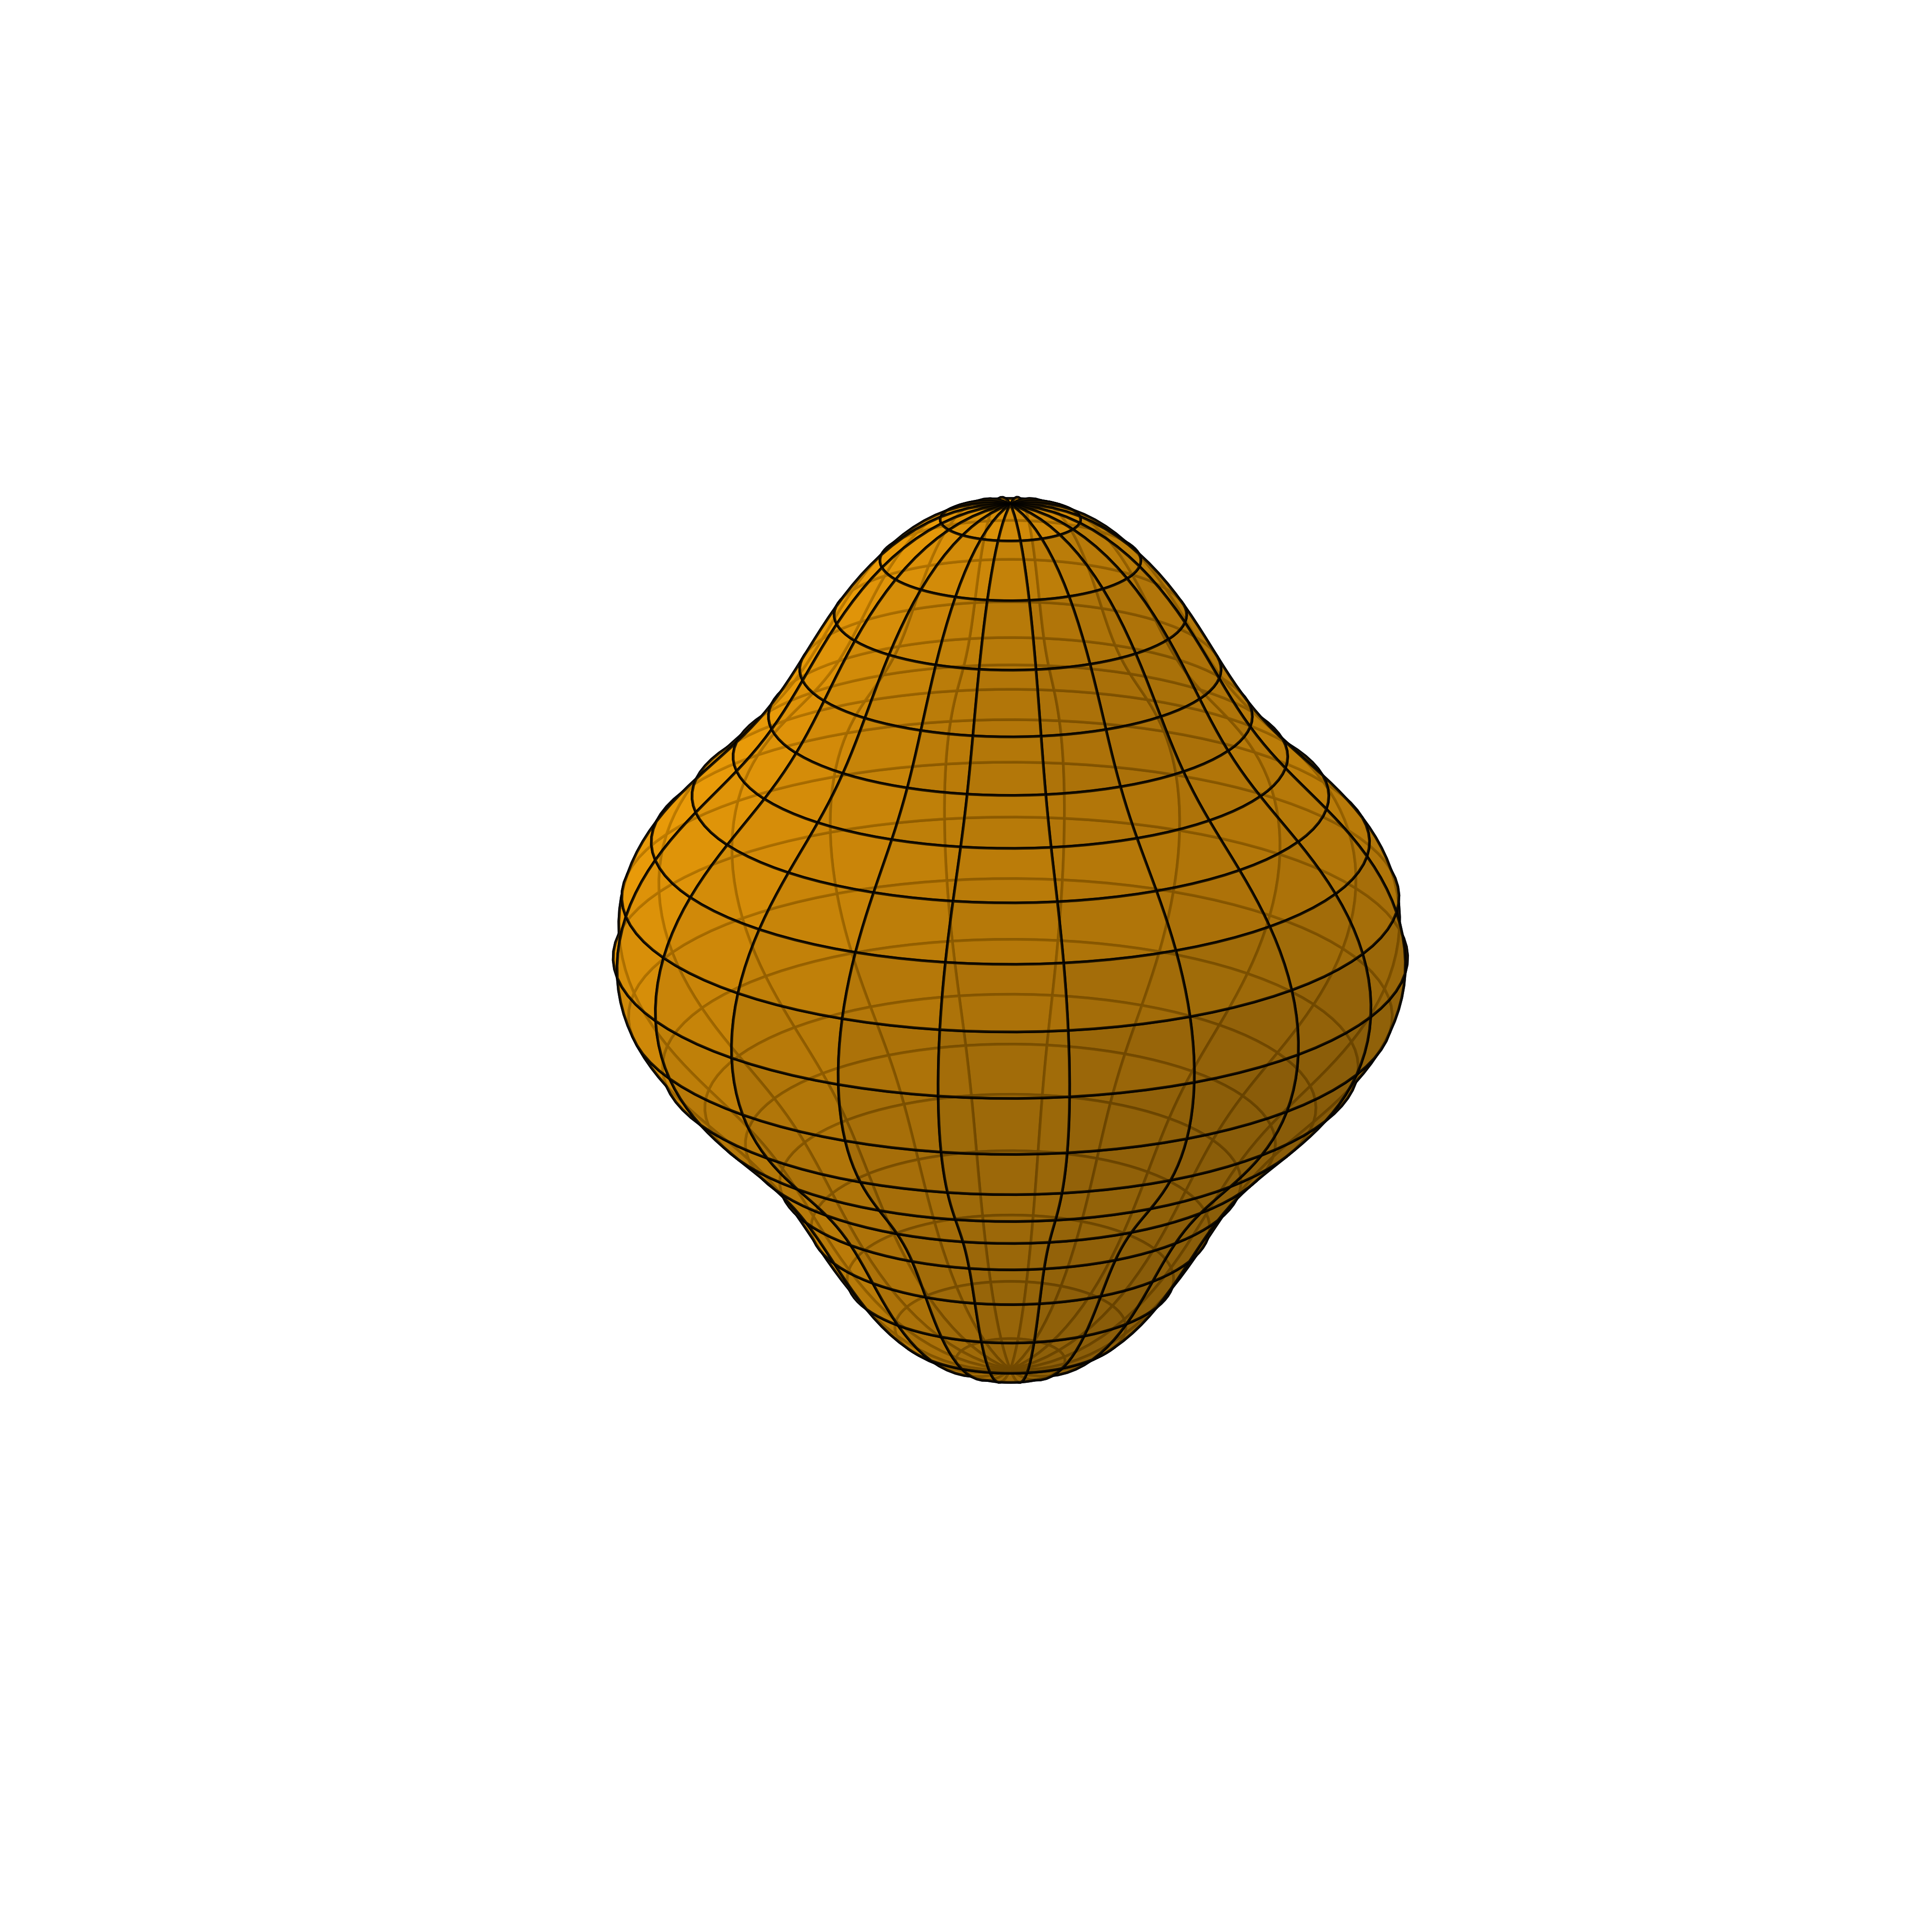
\includegraphics[width=0.25\linewidth]{figs/node_0_25.png}
  \caption{Our new nodal surface.}\label{fig:node}
\end{figure}

\end{itemize}
\end{frame}


\begin{frame}{Nodal Errors (IV)}
\begin{figure}[H]
  \centering
  \includegraphics[width=0.7\linewidth]{figs/ell_node_plot.pdf}
  \caption{DMC energies of $\psi^{\alpha,
  \gamma}_{2S}$.}\label{fig:ell_node_plot}
\end{figure}

\begin{itemize}

  \item Conversely with Fig.~\ref{fig:2s_node}, the nodal error is
  \blue{positive}.

\end{itemize}
\end{frame}


\begin{frame}{Nodal Errors (V) - The Point}
\begin{itemize}

  \item Nobody should pretend that the nodal errors we have discussed here are
  \blue{realistic} or general in any way.

  \item This has been a toy model which illustrates something very important.

  \item \red{Never} optimise parameters that affect the nodal surface in a
  trial excited state - \blue{unless} you are certain that the trial wave
  function has the important symmetry properties.

\end{itemize}
\end{frame}


\subsection{Finite Size Effects}\label{sub:fs_effects}
\subsubsection{Single-particle Finite Size Effects (SPFSE)}\label{subsub:spfe}

\begin{frame}{Single-particle Finite Size Effects}
\begin{itemize}

  \item In common with GS calculations, finite size (FS) effects are often
  \blue{very important} in excited state calculations.

  \item ``Single-particle FS effects'' are those related to momentum
  quantisation: the things that we would usually want to twist average over.

  \item {\bf Question:} Do SPFSE affect excited-state calculations?

\end{itemize}
\end{frame}


\begin{frame}{SPFSE (II)}
\begin{itemize}

  \item {\bf Answer:} Apparently not much\ldots we have tested this in InSe
  (2D) and bulk silicon (3D), finding that energy gaps and quasiparticle energy
  bands are rather flat for different values of ${\bf k}$.

\end{itemize}

% \begin{figure}[H]
%   \centering
%   \includegraphics[width=0.8\linewidth]{figs/si_hh_band.pdf}
%   \caption{The heavy hole band in Si, calculated along the line
%   $\Gamma \rightarrow X$.}
% \label{fig:si_hh_band}
% \end{figure}

\begin{figure}[H]
  \floatbox[{\capbeside\thisfloatsetup{capbesideposition={left, center},
  capbesidewidth=0.2\textwidth}}]{figure}[\FBwidth]
  {\caption{The heavy hole band in Si, calculated along the line $\Gamma
  \rightarrow X$}\label{fig:si_hh_band}}
  {\includegraphics[width=0.8\textwidth]{figs/si_hh_band.pdf}}
\end{figure}
\end{frame}

\begin{frame}{``Twist averaging'' Energy Gaps}{Credit NDD}
\begin{itemize}

  \item Choose a point of interest, ${\bf k}_e$, and a twist, ${\bf
  k}_s$.\footnote{\ The point ${\bf k}_e$ is supposed to be a band minimum in
  this case.}

  \item Calculate GS energy, ${E_{0} ({\bf k}_e+{\bf k}_s)}$.

  \item Calculate addition energy, $E^{+} ({\bf k}_e+{\bf{k}_s})$.

  \item Calculate electron-like band,
  \begin{equation}
    \mathcal{E}({\bf k}_e + {\bf k}_s) = E^{+}({\bf k}_e + {\bf k}_s) -
    E_{0}({\bf k}_e + {\bf k}_s) \nonumber,
  \end{equation}
  \item Repeat for desired number of twists. Fit data,
  \begin{equation}
    \mathcal{E}({\bf k}_e + {\bf k}_s) = \mathcal{E}_{\text{TA}}({\bf k}_e) +
    {\bf k}_s \cdot (\mathrm{A}{\bf k}_s) \nonumber,
  \end{equation}
  \item Ultimately, this yields a (TA) \green{QMC energy band value}, and a
  \green{QMC effective mass}.\footnote{\ This effective mass can
  be extracted from the matrix $\mathrm{A}$, which is an effective ``band
  curvature tensor''.}

\end{itemize}
\end{frame}


\subsubsection{Many-body FS Effects}\label{subsub:mb_fs_effects}

\begin{frame}{Many-body FS Effects (MBFSE)}{Specific to solids\ldots}

\begin{itemize}

  \item Excited state calculations carry more a \red{far more potent} class of
  finite size errors.

  \item Consider adding an electron to a simulation supercell. $N_e \rightarrow
  N_e + 1$, and a neutralising background is added to maintain charge
  neutrality.

\begin{minipage}[t]{0.4\textwidth}

  \only<1>{\centering\includegraphics[width=0.9\linewidth]{figs/sc_1.pdf}}
  \only<2>{\centering\includegraphics[width=0.9\linewidth]{figs/sc_2.pdf}}
  \only<3>{\centering\includegraphics[width=0.9\linewidth]{figs/sc_3.pdf}}
  \only<4>{\centering\includegraphics[width=0.9\linewidth]{figs/sc_4.pdf}}

\end{minipage}%
\hfill
\begin{minipage}[t]{0.5\textwidth}
\vspace{-4.0cm}
\begin{itemize}

  \item UC = 1 square, SC = $2\times2\times p$ grid. \pause{}

  \item Added a quasiparticle to one unit cell. \pause{}

  \item By translational invariance, there are others! \pause{}

  \item Neutralising background added.

\end{itemize}
\end{minipage}%
\end{itemize}
\end{frame}


\begin{frame}{MBFSE (II)}
\begin{itemize}

  \item These charges interact with the system (as we want them to\ldots),
  \red{but} they also interact with themselves.

  \item This happens in the ground state case, and such ``self-terms'' are
  subtracted in the \blue{Madelung constant}.

  \item Here, the leading order correction to the excited state energy is the
  Madelung constant for particles in neighbouring supercells, interacting
  \blue{in the effective medium supplied by the rest of the
  system}.\footnote{\ The interactions between added/removed quasiparticles are
  {\bf screened} by the rest of the system.}

  \item This has been studied before, in the context of DFT defect
  energetics.\footfullcite{Murphy2013}

\end{itemize}
\end{frame}


\begin{frame}{MBFSE (III)}
\begin{itemize}

  \item I recently found that screened Madelung constants can be
  evaluated \green{as they are in the unscreened case}, if you transform
  variables.\footnote{\ The idea is to move to the principal axis of the
  dielectric tensor, and to then scale it to the identity matrix. These
  transformations manifest in a Jacobian, and can be undone to yield a
  screened $v_{\text{M}}$.}

  \item The Madelung constant for a set of charges in a material with
  ``background'' dielectric tensor $\tilde \epsilon$ is
  \begin{equation}
    v^{\text{Scr.}}_{\text{M}}({\bf R}) \rightarrow
    \dfrac{1}{\sqrt{\det{\left[ \tilde \epsilon \right]}}}
    v^{\text{Unscr.}}_{\text{M}}(\sqrt{\tilde\epsilon^{-1}} {\bf R}),
  \end{equation}
  where ${\bf R}$ represents the matrix of supercell lattice vectors.

\end{itemize}
\end{frame}

\begin{frame}{MBFSE (IV)}

\begin{itemize}

  \item This looks \red{sketchy}\footnote{\ For example, which square
  root do I take?} but in actual fact the restrictions on $\tilde\epsilon$ mean
  this is a well defined operation.

  \item The ability to use anisotropically screened Coulomb interactions in
  \textsc{casino} is a \green{planned feature}.

  \item What use would this have?

  \begin{itemize}

  \item Study model systems of electrons and holes in an anisotropically
  screened environment.

  \item ``On-the-fly'' \blue{corrections} for QMC gap calculations.

  \item Qualitative study of FS effects in calculations of real materials -
  e.g.\ how are FS effects \blue{qualitatively different} (scaling-wise) in
  cubic vs.\ hexagonal systems?


  \end{itemize}
\end{itemize}
\end{frame}


\begin{frame}{MBFSE (V)}

\begin{block}{Example: electronic addition calculation}

\begin{itemize}
  \item The relevant quantity here is the ``quasiparticle band energy''
  \begin{equation}
    E_{\text{e-QP}} = E^{0}_{N+1} - E^{0}_{N},
  \end{equation}
  which ought to be corrected. We need to \blue{remove} the energy of a lattice
  of quasi-electrons interacting in a medium determined by the ``rest of the
  system''.
  \begin{equation}
    E^{\text{corr.}}_{\text{e-QP}} = E_{\text{e-QP}} -
    \dfrac{v^{\text{Scr.}}_{M}}{2}.
  \end{equation}
\end{itemize}
\end{block}
\end{frame}


\begin{frame}{MBFSE (VI) - Excitonic FS Effects}
\begin{itemize}

  \item In the case of a promotion calculation, the FS effects \red{are not}
  due to interacting (single) quasiparticles and their compensating background.

  \item These FS effects can scale \blue{differently} with system size.

  \item There seems to be no general statement to be made here (we are still
  working!), however, corrections are usually \blue{extrapolated}, with
  $\mathcal{O}(N_e^{-p})$ corrections accounted for in fitting.

  \item The exponent $p$ \blue{changes on a study-by-study basis}, depending on
  dimensionality, the nature of the excitation ((de)-localised?), the size of
  the simulation cell, \ldots

\end{itemize}
\end{frame}


% \begin{frame}{Excitonic FS Effects: An example}
%
% [TO BE ADDED, OR NOT]
% \begin{itemize}
%   \item Will contain some wrangling of fitting exponents ($p$), effectively
%   taken from the BN gap paper FS section.
%
% \end{itemize}
%
% \end{frame}


\begin{frame}{Finite Size Effects: A Brief Summary}

\begin{itemize}
  \item FS effects \red{alter the numbers} we get out of excited state
  calculations at different (fixed) system sizes.

  \item We should try to remove them (e.g.\ with $v^{\text{Scr.}}_{\text{M}}$),
  but \blue{usually also need to extrapolate} in order to reach the
  thermodynamic limit.

  \item FS effects are the \red{dominant source of error} in excited state QMC
  calculations of solids.

  \item \green{None of the nasty FS effects we're currently having trouble with
  affect calculations on aperiodic (truly finite) systems.}\footnote{\ In this
  case, ``FS effects'' correspond to \textit{physical phenomena}, e.g.\ quantum
  confinement.}

\end{itemize}
\end{frame}

% }}*

% *{{ Examples
\section{Examples}\label{sec:examples}

\subsection{Atoms and Molecules}\label{sub:atoms_and_molecules}

\begin{frame}{Examples: Atoms and Molecules}{Let's talk about aperiodic
systems!}

\begin{itemize}
  \item Obviously, we have \green{no problem} with FS effects here.
  \item We do, however, \blue{potentially} have other problems:
  \begin{itemize}
    \item Nodal error
    \item Vibrational effects (I'll include static Jahn-Teller\footnote{\ One can
    imagine that excited states may suffer a JT distortion - which means we
    should, in principle, consider the ground and excited state molecular
    geometries when doing QMC calculations.} effects here)
    \item Pseudopotential-induced error
  \end{itemize}

  \item It would be nice to have a handle on these issues, and to know whether
  or not excited state QMC is any good for these kinds of systems.

\end{itemize}
\end{frame}


\begin{frame}{The Ne atom}

\begin{itemize}
  \item The Neon atom and its first ionization potential have been studied
  before (by some people in the room).\footfullcite{Drummond2006}

  \item There's other work which seems to uncover a general fact about nodal
  errors in atomic systems: they scale $\sim$ linearly with electron
  density.\footfullcite{Rasch2012}

  \item {\bf Question:} Do nodal errors build up in the $n^{\text{th}}$
  ionization potentials, as well as the energies?\footnote{\ I.e.\ does the
  strength of this growth in nodal error matter on the scale of an IP?}
\end{itemize}
\end{frame}


\begin{frame}{The Ne atom: results}

\begin{itemize}
  \item By successively removing electrons from the Ne atom, we obtain the
  following table of results,

\end{itemize}

\begin{table}[H]
  \centering
  \begin{tabular}{cccccc}
$n$ & Exact NR IP & SJ-VMC & SJB-VMC & SJ-DMC & SJB-DMC  \\ \hline
 1 & 21.61333 & 22.08(2)  & 21.96(2)  & 21.72(1)  & 21.72(1)  \\
 2 & 40.99110 & 41.48(2)  & 41.39(2)  & 41.10(1)  & 41.06(1)  \\
 3 & 63.39913 & 63.44(2)  & 63.23(1)  & 63.35(2)  & 63.39(1)  \\
 4 & 97.29312 & 97.91(2)  & 97.78(1)  & 97.75(2)  & 97.72(1)  \\
 5 &126.28846 & 126.85(2) & 126.72(2) & 126.85(1) & 126.79(1) \\
 6 &157.80001 & 158.43(2) & 158.30(1) & 158.25(2) & 158.34(1) \\
 7 &207.04137 & 204.48(2) & 204.56(1) & 205.04(2) & 205.26(1) \\
 8 &238.78949 & 238.10(1) & 238.49(1) & 238.70(2) & 238.79(1) \\
 \hline
 { }& Avg. MAE & \textcolor{red}{0.83\%}    & \textcolor{BurntOrange}{0.67\%}
 & \textcolor{ForestGreen}{0.38\%}    & \textcolor{green}{0.34\%}

  \end{tabular}
  \caption{QMC vs.\ a set of ``Exact NR IP''
  values, in eV.\footfullcite{Chakravorty1993}}\label{tab:neon_ips}
\end{table}
\end{frame}


\begin{frame}{Miscellaneous Molecules}
\begin{itemize}
  \item Molecules are one step up from atoms: structural/vibrational effects
  can be important.\footfullcite{Mostaani2016}

  \item As a test of QMC, we have studied the ionization potentials / electron
  affinities of various small molecules.
\noindent\mbox{
\begin{minipage}[t]{0.48\textwidth}
  \begin{itemize}
    \item Tetracyanoethylene
    \item Boron trifluoride
    \item H$_2$/O$_2$
    \item Benzothiazole
    \item Anthracene
  \end{itemize}
\end{minipage}%
\hfill
\begin{minipage}[t]{0.48\textwidth}
\vspace*{\fill}
\begin{align}
  \text{IP} &= E_{N-1} - E_{N} \nonumber \\
  \text{EA} &= E_{N} - E_{N+1} \nonumber
\end{align}
\vspace{0.2cm}
\item  3 energies to be calculated. All obey ``ground-state'' variational
principles.
\vspace*{\fill}
\end{minipage}}%
\end{itemize}
\end{frame}


\begin{frame}{Misc. Molecules (II)}
\begin{itemize}
  \item These calculations are so cheap, we can do them with a PW basis and at
  various levels of QMC expense:\@ SJ-VMC, SJB-VMC, SJ-DMC, SJB-DMC.\@

  \item Testing multi-determinant wave functions is also probably feasible. But
  this is tricky/distasteful. Why?

  \item We would like our wave function parametrisation to be \green{compact},
  and to have the property that it retrieves correlation energy
  \green{efficiently}.

  \item Excited state multi-determinant expansions \red{require care} in
  preparation.  Variational principles become (again) \red{more
  complicated}.\footnote{\ Granted, this is not the case for IP/EA calculations.}

\end{itemize}
\end{frame}


\begin{frame}{Tetracyanoethylene (TCNE)}
\begin{itemize}
 %\item TCNE is one of those molecules theorists can \green{happily} work with.
 %Experimentalists \red{not so much}.

  \item TCNE is an electron acceptor, with an EA of 3.16(2)
  eV.\footfullcite{Khuseynov2012}

  \item (Aged) experiments determine IP $\sim$ 11.67-11.79 eV.
\end{itemize}

\vspace{-0.9cm}
\begin{minipage}[t]{0.4\textwidth}

\begin{figure}[H]
  \centering
  \includegraphics[width=0.7\linewidth]{figs/tet.png}
  \caption{TCNE}\label{fig:tet}
\end{figure}

\end{minipage}%
\hfill
\begin{minipage}[t]{0.5\textwidth}

\begin{table}[H]
  \centering
  \begin{tabular}{ccc}
  Method  & IP / eV  & EA / eV \\ \hline
  SJD     & 11.87(1) & 3.23(1)  \\
  SJD-JT  & 11.85(1) & 3.25(1)  \\
  SJBD    & 11.88(1) & 3.20(1)  \\
  SJBD-JT & 11.86(1) & 3.23(1)  \\ \hline
  CCSD (T) & 11.99 & 3.05 \\
  $GW$    &?? &?? \\
  SCQP$GW$&?? &??
  \end{tabular}
  \caption{EA/IP values of TCNE.}\label{tab:label}
\end{table}

\end{minipage}%

\begin{itemize}
  \item Errors: PP \& dynamical vibrational effects.
\end{itemize}

\end{frame}

\begin{frame}{Other Misc. Molecules: A Quick Slide}

\begin{itemize}
  \item How do we generally do, for small molecules and compared to
  $GW$, etc?
\end{itemize}

\begin{table}[H]
\centering
\caption{EA/IP values (in eV) of some more molecules.}\label{tab:molecules}
\begin{tabular}{ccccccc}
 & \multicolumn{2}{c}{BF$_3$} & \multicolumn{2}{c}{Anthracene} &
 \multicolumn{2}{c}{Benzothiazole} \\
Method & IP      & EA      & IP      & EA      & IP      & EA      \\
SJD    &16.226(6)& --      & 7.35(3) & 0.33(3) & 8.94(2) & 0.67(2) \\
SJD-JT &16.227(6)& --      & 7.31(3) & 0.45(3) & 8.80(2) & 0.54(2) \\
$GW$   &  --     & --      & 7.06    & 0.32    & 8.48    & --      \\
SCQP$GW$& --     & --      & --      & --      & 8.83    & --      \\
CCSD (T)& --     & --      & 7.52    & 0.33    & 8.70    & --      \\
Expt.  & 15.7(3) & --      & 7.439(6)& 0.53(2) &$\tilde{8.8}$& --
\end{tabular}
\end{table}
\end{frame}


\begin{frame}{Recap of references}{Because I'm a good boy}
\begin{itemize}
  \item I haven't listed all of the references for my comparison data on the
  relevant slides because there are \red{too many}.

  \item In the interest of being \green{good} their numbers (see References
  slides) are:

  \begin{itemize}
    \item CCSD (T) reference data.\footfullcite{Richard2016}

    \item $GW$ for anthracene,
    benzothiazole.\footfullcite{Blase2011}\footnote{\ EA not quoted, but IP and
    HOMO-LUMO gap are. Do the maths.}

    \item SCQP$GW$ benzothiazole.\footfullcite{Kaplan2016}

    \item Experiments: mostly from NIST web
    pages.\footfullcite{Nist2005} The value with a tilde is an average of the
    available (fairly varied) experimental IP data.
  \end{itemize}
\end{itemize}
\end{frame}


\subsection{Solids}\label{sub:solids}

\begin{frame}{Solids}

\begin{itemize}

  \item I'll give two brief examples here. The first two projects have been
  very illuminating for us - I'll aim to \green{share some wisdom} here.

  \begin{itemize}
    \item Silicon: old and new
    \item Boron Nitride: from bulk to monolayer
    \item Fermi Liquid Theory: what can QMC say?

  \end{itemize}
\end{itemize}
\end{frame}


\begin{frame}{Solids: A Quickfire How-To}

\begin{enumerate}
  \item Select supercell sizes / supercell matrices (this determines, by the
  many-body Bloch conditions, the {\bf k}-point grid). In symmetrical cases, one
  probably wants to specify less {\bf k}-points (file sizes).
  \begin{itemize}
    \item Can you study the excitations you want with the {\bf k}-points you
    are now forced to use? This is not always the case.
    \item Check your pseudopotentials (TM ions are the
    worst).\footfullcite{Drummond2016}
  \end{itemize}
  \item Obtain single-particle orbitals - PW DFT or Gaussian basis DFT.\@ Plane
  waves if HEG.\@
  \item Check time step biases in some trial excited states - possible to make
  savings here! (we haven't exploited this fully yet!)
  \item Run calculations, reconvene to worry about FS effects some time
  later\ldots
\end{enumerate}
\end{frame}


\begin{frame}{Silicon: the 90s}
\begin{itemize}
  \item In the 90s, an early set of QMC calculations for silicon did something
  interesting\ldots
  \item Using excitonic SJ wave functions (as introduced earlier), Williamson
  \textit{et al.}\footfullcite{Williamson1998} mapped out the band structure of
  silicon at high symmetry points.
\end{itemize}
\begin{figure}[H]
  \floatbox[{\capbeside\thisfloatsetup{capbesideposition={left, center},
  capbesidewidth=0.6\textwidth}}]{figure}[\FBwidth]
  {\caption{Band structure at HS points (dots) in silicon, ca. 1998. Solid
  lines are PP calculations. This was calculated for a $2\times2\times2$
  supercell of silicon.}\label{fig:si_bs_90s}}
  {\includegraphics[width=0.3\textwidth]{figs/si_bs_90s.png}}
\end{figure}
\end{frame}


\begin{frame}{Silicon: Now}
\begin{itemize}
  \item Owing to the heightened availability of computational resources,
  various aspects of the previous work can be improved on.
  \begin{itemize}
    \item Lower statistical errors.
    \item \blue{Finite size effects}.
    \item BS away from HS points (see earlier hole band!).
  \end{itemize}
  \item Our ongoing work considers the quasiparticle and excitonic gaps in
  silicon, at various system sizes.
  \begin{align}
    \Delta_{\text{QP}} &= E_{N+1} + E_{N-1} - 2E_{N} \nonumber, \\
    \Delta_{\text{EX}} &= E^{\star}_{N} - E_{N}.
  \end{align}
  \item If DMC were not pathological (\& it isn't!), we'd expect to be able to
  take both to the thermodynamic limit and obtain $\Delta_{\text{QP}} \sim
  \Delta_{\text{EX}}$.
\end{itemize}
\end{frame}


\begin{frame}{Silicon: Maybe next time}
\begin{itemize}
  \item We don't actually know if this is true yet ($2\times2\times2$ \&
  $3\times3\times3$ results are encouraging).
  \item Stay tuned.
\end{itemize}

\begin{block}{What do we know?}
  \begin{itemize}
    \item Single-particle FS effects \green{don't play much of a role}.

    \item QP gap has \red{more severe} FS effects.
    (has ramifications for other cases where excitonic effects are
    \blue{weak}).

    \item We are probably \red{limited} to an error bar of $\sim$ 0.1 eV,
    thanks to PPs.\footnote{\ Even if we had a perfect theory of FS effects. In
    this (cubic) system, this might be less of a pain.}

    \item \textbf{Question:} How do we know all of this?
  \end{itemize}
\end{block}
\end{frame}


\begin{frame}{Hexagonal Boron Nitride}
\begin{itemize}
  \item We have spent far more time on a related project, where our goal is to
  calculate the excitonic and quasiparticle gaps of hBN.\@
  \begin{itemize}
    \item \blue{Large} gap insulator (bulk and monolayer).

    \item Anisotropic dielectric properties (non-diagonal $\tilde\epsilon$).

    \item \green{Extremely} interesting to experimentalists.

    \item We know almost \red{nothing}\footnote{\ Nothing correct, that is.
    Sorry DFT.} about the electronic properties of the monolayer.
  \end{itemize}
\end{itemize}
\end{frame}


\begin{frame}{HBN:\ What have we done?}
\begin{itemize}
  \item We've studied a series of bulk and monolayer system sizes (``square''
  supercells in the monolayer, ``spherical'' in the bulk - \blue{maximal WS
  radius}).
  \item We have calculated the QP and EX gaps at various high symmetry points,
  with a goal of extracting \blue{exciton binding energies} from first
  principles
  \begin{equation}
    E^{X}_{B} = \Delta_{\text{QP}} - \Delta_{\text{EX}}.
  \end{equation}
  \item This would offer a QMC alternative to $GW$-BSE
  approaches.\footnote{\ This is the only competitor method, and has its
  own problems.}
\end{itemize}
\end{frame}


\begin{frame}{HBN:\ Results}{Monolayer}
\begin{itemize}
  \item The monolayer results appear quite well-behaved, but feature
  quasi-random FS errors of order 0.1 eV.
\begin{figure}[H]
  \floatbox[{\capbeside\thisfloatsetup{capbesideposition={left, center},
  capbesidewidth=0.4\textwidth}}]{figure}[\FBwidth]
  {\caption{Energy gaps in monolayer hBN as a function of system
  size}\label{fig:monolayer_gaps}}
  {\includegraphics[width=0.5\textwidth]{figs/monolayer_gaps.pdf}}
\end{figure}
\end{itemize}
\end{frame}


\begin{frame}{HBN:\ Results}{Monolayer cont.}
\begin{itemize}
  \item We predict a \textit{vacuum} exciton binding of 2.0(4) eV, which is
  comparable to $GW$-BSE (2.1 eV).\footfullcite{Wirtz2006} Both of these ought
  to be modulated by the particular dielectric environment.
  \item Experimental comparison (when possible) must be done taking into
  account the fact that we have \textit{vacuum} results. Our results are
  \blue{renormalised strongly} if $\epsilon \neq 1$.
\end{itemize}
\end{frame}


\begin{frame}{HBN:\ Results}{Bulk}
\begin{itemize}
  \item After correction ($v^{\text{Scr.}}_{\text{M}}$), some gaps OK.\
  Have the same $\mathcal{O}(0.1\ \text{eV})$ quasi-random FS errors as
  the monolayer.\footnote{\ In the best case. $K \rightarrow K$ not the best
  case\ldots Generally, the FS effects are a lot worse in the bulk, especially
  where bands are flat.}
\begin{figure}[H]
  \floatbox[{\capbeside\thisfloatsetup{capbesideposition={right, center},
  capbesidewidth=0.3\textwidth}}]{figure}[\FBwidth]
  {\caption{Energy gaps in bulk hBN as a function of system
  size.}\label{fig:bulk_gaps}}
  {\includegraphics[width=0.7\textwidth]{figs/bulk_gaps.pdf}}
\end{figure}
\end{itemize}
\end{frame}


\begin{frame}{HBN:\ Loose Ends}
\begin{itemize}
  \item We are investigating the sources of this quasi-random error, which
  seems also to affect InSe (monolayer), and phosphorene.
\end{itemize}
\begin{block}{Things that apparently don't matter $\left[\text{at }
\mathcal{O}(0.1\text{eV}) \right]$}
\begin{itemize}
  \item SPFS effects (energy gap landscape as fn.\ of ${\bf k}_s$ is flat)
  \item (DFT) Dielectric tensors at ``fixed cell sizes'' vs.\ expt.\ ones.
  \item Variational principles: this is common to QP and EX gaps, and the only
  candidates\footnote{\ We use complex wave functions for some of our gaps at
  K, and take care to re-calculate ground state energies with the shifted
  grids.} for broken VPs are data points where an increase in the gap would
  seem to make the situation worse.
  \end{itemize}
\end{block}
\end{frame}


\begin{frame}{Excited States in Metals: Fermi Liquid Theory}
\begin{itemize}
  \item A normal metal can (generically) be described by \blue{Fermi liquid
  theory}.
  \item The excitations of such a system can be considered to be
  ``almost free'' quasiparticles\footnote{\ This follows from the idea that
  the interacting ground state is \textit{adiabatically connected} to the
  non-interacting one.} - they are quasielectrons with a
  \textit{renormalised} effective mass, and whose interactions are
  characterised by a set of numbers (Landau's interaction parameters).
  \item QMC has been used to say something quantitative about this description.
  \item (Of course, these kinds of excitations only dominate at low
  temperature, at higher temperature, others can interfere. Collective
  modes may exist, for example.)
\end{itemize}
\end{frame}


\begin{frame}{Fermi Liquid Theory (II) - The Language and Ideas of FLT}

\begin{itemize}
  \item What is the deviation from the non-interacting ground-state energy,
  $\delta E$, due to the presence of quasiparticles?
  \item Let $\delta n_{\bf k,\sigma} = n_{\bf k,\sigma} - n^{0}_{\bf
  k,\sigma}$, and work on the assumption that $\delta n$ is small. The energy
  can be expanded
  \begin{equation}
    E\left[ \delta n \right]= E^{0} +
    \underbrace{\sum_{\bf k,\sigma} \epsilon_{\bf
    k,\sigma}\delta n_{\bf k,\sigma}}_{\text{QP KE}} +
    \underbrace{\sum_{\bf k,\sigma} \mathcal{F}_{\bf
    k \bf q,\sigma \tau}\delta n_{\bf k,\sigma} \delta n_{\bf
    q,\tau}}_{\text{QP Int. E.}} + \mathcal{O}\left[{(\delta n_{\bf
    k\sigma})}^3\right].
  \end{equation}
  \item In practice, the $\mathcal{F}$'s are restricted by {isotropy} and
  \green{symmetry} arguments, but I won't focus on them here. Instead I'll focus on the
  \blue{quasiparticle kinetic energies}.
  \item This term describes the kinetic energy of the quasiparticles of the
  interacting system, whose effective mass is \textit{renormalised} by
  e-e interactions.
\end{itemize}
\end{frame}


\begin{frame}{Fermi Liquid Theory (III) - Effective Masses}
\begin{itemize}
  \item The dispersion relation of quasiparticles close to the Fermi energy
  ($\epsilon_F$) can
  be taken to be
  \begin{equation}
    \epsilon_{\bf k,\sigma} = \epsilon_F + \dfrac{k_F}{m^{\star}}(k - k_F),
  \end{equation}
  where $m^{\star}$ is the \textit{quasiparticle effective mass}.\footnote{\
  This can be of order $m_e$, however, it can also exceed $10^3 m_e$ (in
  so-called ``heavy fermion'' materials).}
  \item I'll now move on to the QMC calculations!
  \item Before I do, lets mention that FLT has the ability to \textbf{predict
  its own death}. If some physics lowers the energy of a competing phase, the
  liquid may be unstable, and this usually signals the dominance of the
  \textbf{new phase}.
  \begin{itemize}
    \item Magnetic instabilities.
    \item Density wave / Pomeranchuk instabilities.
  \end{itemize}
\end{itemize}
\end{frame}


\begin{frame}{Fermi Liquid Theory - What Can QMC Say?}

\begin{itemize}
  \item QMC for the HEG can be used to explicitly calculate $\epsilon_{\bf
  k,\sigma}$ in the (para- and ferr-)\@magnetic case. I.e.\ we can extract the
  leading term of the Landau functional, $E\left[ \delta n  \right]$.
  \item Using SJB wave functions, Neil Drummond and Richard Needs have studied
  the HEG, and extracted quasiparticle effective masses.\footfullcite{Drummond2013}
  \begin{itemize}
    \item Optimize GS wave function.
    \item Add or remove electrons.
    \item Calculate energy band $\epsilon_{\bf k}$.
    \item Rinse and repeat for systems of varying density and size.
  \end{itemize}
\end{itemize}
\end{frame}

\begin{frame}{Fermi Liquid Theory - What Can QMC Say? (II)}
\begin{figure}[H]
    \centering
    \begin{subfigure}[c]{0.48\textwidth}
        \includegraphics[width=0.7\textwidth]{figs/masses.pdf}
        \caption{$m^{\star}$ versus system size.}\label{fig:masses}
    \end{subfigure}
    \begin{subfigure}[c]{0.48\textwidth}
        \includegraphics[width=0.6\textwidth]{figs/bands-cropped.pdf}
        \caption{[crop] $\epsilon_{\bf k}$ versus system size.}\label{fig:bands}
    \end{subfigure}
    \caption{Both from earlier referenced study.}\label{fig:masses_bands}
\end{figure}
\vspace*{-0.5cm}
\begin{itemize}
  \item This is another example where the biting point for QMC calculations of
  excited state is made clear: \red{Finite Size Effects!}\footnote{\ At high
  $r_s$, at least.}
\end{itemize}
\end{frame}

% }}*

% *{{ To-Dos for Excited State QMC
\section{Wisdom for Excited State DMC Calculations}\label{sec:wisdom}
\begin{frame}{Wisdom for Excited State DMC Calculations}

\begin{itemize}
  \item \green{Do} investigate systematic biases, and try to exploit them.

  \item \green{Do} assess project feasibility before starting: some gap
  calculations are forbidden by supercell size/shape. Some materials have large
  unit cells.

  \item \green{Do} be careful when carrying out calculations: check band
  occupancies, regenerate blip binaries, \ldots

  \item \green{Do} respect GS wisdom!

  \item \red{Don't} optimize parameters that affect the nodal surface in trial
  excited states.\footnote{Unless you are \textbf{sure}. In our limited tests,
  we find that backflow has little effect on excited state energy gaps anyway.}

  \item \red{Don't} waste time lowering statistical error bars beyond the
  limits of accuracy (set by FS effects, in solids).

\end{itemize}

\end{frame}

% }}*

% *{{ Thanks!
\begin{frame}[plain]
\begin{center}
  {\Huge Thank you all for listening!} \\
  %\vspace{2cm}
  %{\Large} Thanks to the NOWNano CDT / EPSRC for my funding.
\end{center}
\end{frame}
% }}*

% - - - - - - - - - - - - - - - - - - - - - - - - - - - - - - - - - - -

% *{{ References and end document
\begin{frame}[t,allowframebreaks]{References}

\printbibliography[]

\end{frame}
\end{document}

% }}*
